% vim:ts=2 sw=2 et spell tw=80:

\section{Applications}
\label{kugel:sec:applications}

As suggested in the previous section, the fact that it is possible to write a
Fourier style expansion of any function on the surface of the sphere is very
useful in many fields of physics and engineering. Here we will present a few of
the most interesting applications we came across during our research.

\subsection{Electroencephalography}

\begin{figure}
  \centering
  \subfigure[EEG Electrodes \label{kugel:fig:eeg-electrodes}]%
    {\includegraphics[width=.45\linewidth]{papers/kugel/figures/electrodes}}
  \qquad
  \subfigure[Gauss' Law \label{kugel:fig:eeg-flux}]%
    {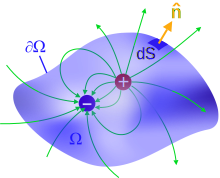
\includegraphics[width=.4\linewidth]{papers/kugel/figures/flux}}
  \caption{
    Courtesy of C. Hope \cite{sheerman-chase_volunteer_2012} for picture (a),
    and Wikimedia \cite{maschen_english_2013} for (b).
    \label{kugel:fig:eeg}
  }
\end{figure}

To start, we will look at an application that is from the field of medicine:
electroencephalography. The \emph{electroencephalogram} (EEG) is a measurement
of the electrical field on the scalp, which shows the brain's activity, and is
used in many fields of research such as neurology and cognitive psychology.  The
measurement is done by wearing a cap that contains a number of evenly
distributed electrodes, each of which measures the electric potential (voltage)
at their location (figure \ref{kugel:fig:eeg-electrodes}).  To see how this will
relate to the spherical harmonics, we will first quickly recap a bit of physics,
electrodynamics to be precise.

\subsubsection{Electrodynamics}
\nocite{griffiths_introduction_2015}

In section \ref{kugel:sec:construction:eigenvalue} we have shown that the
spherical harmonics arise from the surface spherical Laplacian operator, whose
origin we did not consider too much, which is how mathematicians do their work.
On the contrary, physicists usually do the opposite and start by discussing what
is happening in the real world, since variables represent physical quantities.
So, we will quickly remind that the Laplacian operator does the following to an
electric potential $\phi(x, y, z)$:
\begin{equation*}
  \nabla^2 \phi
  = \nabla \cdot \nabla \phi
  = \nabla \cdot \mathbf{E}
  = \frac{1}{\varepsilon} \rho,
  \quad \text{or} \quad
  \iiint_\Omega \nabla \cdot \mathbf{E} \, dv
  = \iint_{\partial \Omega} \mathbf{E} \cdot d\mathbf{s}
  = \frac{1}{\varepsilon} \Phi.
\end{equation*}
Put into words: on the left we have the differential form, where we recall that
the Laplacian (which is a second derivative) is the divergence of the gradient.
Unpacking the notation we first see that we have the gradient of the potential,
which is just the electric field $\mathbf{E}$, and then the divergence of said
electric field is proportional to the charge density $\rho$. So, the Laplacian
of the electric potential is proportional to the charge density! For those that
are more familiar with the integral form of Maxwell's equation, we have also
included an additional step using the divergence theorem, which brings us to the
electric flux $\Phi$, which by Gauss' law (shown in the iconic\footnote{Every
electrical engineer has seen this picture so many times that is probably burnt
in their eyes.} figure \ref{kugel:fig:eeg-flux}) equals the net electric charge.

Now, an important observation is that if we switch to spherical coordinates, the
physics does not change. So, the spherical Laplacian $\sphlaplacian$ of the
electric potential $\phi(r, \vartheta, \varphi)$ is still the charge density (in
spherical coordinates). And what about the surface spherical Laplacian
$\surflaplacian$? To that case the physics is also indifferent, the only change
is that the units result is a \emph{surface} charge density $\rho_s$. Thus, we
are done with physics and finally arrive at the engineers' perspective: how can
we use this fact to build something that reads the current flows on the surface
of the brain?

\subsubsection{EEG as Interpolation Problem}

The details of how EEG actually works gets very complicated very quickly, but we
will try our best to give an broad overview of the mathematical machinery that
makes it possible to measure brain waves. The problem neither the physicist nor
the mathematician considered is that we cannot measure the electric field in its
entirety. As show in figure \ref{kugel:fig:eeg-electrodes} the electrodes give
measurements that are only available at discrete locations, and we are thus
missing quite a lot of data. Or in other words, we have an interpolation
problem, which (at this point not so surprisingly) we will show can be solved
using the spherical harmonics.

To solve this new interpolation problem, we will start with a blatantly
engineering assumption: the human head is a sphere of radius $R$, with the value
of $R$ being the average radius of a human head (which is around 11 cm). So, we
will assume that the potential distribution on the head can be written as a
finite linear combination of spherical harmonics:
\begin{equation*}
  V(\vartheta, \varphi)
    = \sum_{n=1}^N \sum_{m=-n}^n a_{m,n} Y^m_n(\vartheta, \varphi),
\end{equation*}
where the values $a_{m,n}$ are the unknowns of our interpolation problem. Now to
the measurements: we let $\phi_1, \phi_2, \ldots, \phi_M$ be the measured voltages
at points in space $p_1, p_2, \ldots, p_M$ (position of the electrodes). To
simplify, we will assume that the electrodes are reasonably evenly distributed,
which means that we have no points that are on top of each other or at wildly
different radii from the origin. With that out of the way, we can now write a
minimization problem:
\begin{subequations}
  \begin{align}
    a_{m,n}^* &= \argmin_{a_{m,n}}
      \int_{\partial S} | \surflaplacian V |^2 \, ds 
      = \int_0^{2\pi} \int_{0}^\pi | \surflaplacian V |^2
        \sin \vartheta \, d\vartheta d\varphi, 
        \label{kugel:eqn:eeg-min} \\
    &\text{under the constraints} \quad V(p_j) = \phi_j
      \quad \text{ for } \quad 1 \leq j \leq M.
      \label{kugel:eqn:eeg-min-constraints}
  \end{align}
\end{subequations}
Essentially, with \eqref{kugel:eqn:eeg-min} we are are asking for the solution
to be smooth by minimizing the square of the total curvature (recall that the
surface spherical Laplacian $\surflaplacian$ is a measure of curvature), while
at the same time with \eqref{kugel:eqn:eeg-min-constraints}, we force the
solution to go through the measured points. The latter is the reason why we
needed to assumed that the measurements are at reasonable locations, something
that (as every engineer show know) is not necessarily the case in the real
world! Thus, to solve this problem, we will use the suspiciously convenient fact
that (hint: eigenvalues)
\begin{equation*}
  \surflaplacian V(\vartheta, \varphi)
    = \sum_{n=1}^N \sum_{m=-n}^n a_{m,n}
      \surflaplacian Y^m_n(\vartheta, \varphi)
    = \sum_{n=1}^N \sum_{m=-n}^n a_{m,n}
      n(n+1) Y^m_n(\vartheta, \varphi).
\end{equation*}
So that when substituted into \eqref{kugel:eqn:eeg-min} results in
\begin{align*}
  \int_{\partial S} \biggl|
    \sum_{n=1}^N \sum_{m=-n}^n n(n+1) a_{m,n}
    Y^m_n(\vartheta, \varphi)
  \biggr|^2 ds
  = \sum_{m, m'} \sum_{n, n'} a_{m',n'} \overline{a_{m,n}}
    n'(n'+1) n(n+1)
    \underbrace{\int_{\partial S} Y^{m'}_{n'} \overline{Y^m_n} \, ds}_{
      \langle Y^{m'}_{n'}, Y^m_n \rangle
    },
\end{align*}
where we used a ``sloppy'' double sum notation to indicate that we have a bunch
of terms of that form. We did not bother to properly expand the product of
double sums, because we can see that at the end we end up with an inner product
$\langle Y^{m'}_{n'}, Y^m_n \rangle$, which as we know equals $\delta_{m'm}
\delta_{n'n}$, so all of the terms where $n' \neq n$ or $m' \neq m$ can be
dropped and \eqref{kugel:eqn:eeg-min} simplifies down to
\nocite{pascual-marqui_current_1988}
\begin{equation}
  a^*_{m,n} = \argmin_{a_{m,n}} 
    \sum_{n=1}^N \sum_{m=-n}^n n^2 (n+1)^2 |a_{m,n}|^2.
\end{equation}

At this point, we could continue solving for an analytical solution to the
minimization problem, for example by differentiating with respect to some
$a_{j,k}$, setting that to zero and so forth, but the job of the spherical
harmonics ends here. So, we will not pursue this further, and instead briefly
discuss a few interesting implications and problems. 

\subsubsection{Sampling, Smoothness and Problems}
\nocite{wingeier_spherical_2001, ruffini_spherical_2002}

The most interesting perhaps unforeseen fact is that with this method we are
getting a free (!) spectral analysis, since the coefficients $a_{m,n}$ are the
spectrum of the interpolated electric potential $V(\vartheta, \varphi)$.
However, like in the non spherical Fourier transformation, we only get a
\emph{finite} resolution since our measurement are spatially discrete. In fact,
if we know the mean angular inter-electrode distance $\gamma$ we can actually
formulate a Nyquist frequency just like in the usual Fourier theory:
\begin{equation}
  f_N = \frac{\pi}{2T}
  \iff
  n_N = \biggl\lfloor \frac{\pi}{2\gamma} \biggr\rfloor.
\end{equation}

Before concluding this overview of EEG, we should point out that in practice
there are about a million problems with this oversimplified approach. We do not
intend to give an in depth explanation (since the authors themselves are not
experts in any of these fields), but there are a few problems that are too big
to ignore, so we will very briefly discuss them now. The first important
real-world problem is that the electrodes are not necessarily at a reasonable
location, so the constraint \eqref{kugel:eqn:eeg-min-constraints} is a bit too
strong, and may end up fitting some noise or disturbances in the measurement. A
simple solution may for example be to introduce a smoothness factor $\lambda >
0$ as follows:
\begin{equation}
  V(\vartheta, \varphi) = \sum_{n=1}^N \sum_{m=-n}^n 
    \frac{a_{m,n}}{1 + \lambda n^2(n+1)^2} Y^m_n(\vartheta, \varphi).
\end{equation}
To find proper smoothness factor $\lambda$, is another problem of its own, thus
we will not discuss it here, since this is getting too long already. Another
important issue is that in the real world, we cannot ``evenly distribute'' the
electrodes on our head. As shown in the image, most of the electrodes are on a
cap, and then there are just a few on the face, and almost none near the jawline
and chin. This is not something that can be ignored, and in fact, makes the
analysis much more difficult. Finally, the most obvious problem is that human
heads are not perfect spheres. Here too, it is possible to account for this fact
and model the head with a more complex shape (for example using the so called
ellipsoidal harmonics) at the cost of making the math quite unwieldy.

\subsection{Measuring Gravitational Fields}

In this section we want to explore a second application of the spherical
harmonics related to the GOCE mission.  The literature does not explain much
concerning the relation between spherical harmonics in the context of
gravitational field measurement, they assume that everybody knows why precisely
these function are used and not for instance some other fancy special function
presented in this book. That is rather understandable because it is a very
specific topic, and it is probably unlikely that anyone reads such documents
without learning first a lot of potential theory. However, we assume that the
average reader does not have this kind of prior knowledge, therefore, in order
to spare you the pain of going through dense physics books \cite{blakely_1995,
hofmann2005physical, griffiths_introduction_2015} (as we had to do) we will
start with a little bit of background before jumping into the core of the
topic\footnote{By the way, the main sources of this section are the books just
cited.  So, those who want some more insight / completeness on these topics can
take a look there.}.

\subsubsection{Geodesy and History}

The term \emph{geodesy} is the name given to the science that is responsible for
answering questions about figure and gravity field of the earth. During this
subsection we will also encounter the \emph{gravitational force}. The relationship
between gravitational force and gravity field (or gravitational field) simply
lies in what we consider to be the reference. The gravitational force only makes
sense if we consider two masses, and the gravitational field is the
gravitational force experienced in a system that has a unit point mass as
reference. For the electrical engineer, this is analogous to the relationship
between the electric field and the \emph{Coulomb force}.

Geodesy started with various scientists, including Newton, that
recognised that the earth could not be a perfect sphere, because of its
rotational movement. To prove this claim as, the scientific method teaches us,
that observations had to be made, which translates into taking measurements on a
planetary scale. As one can imagine, with the technology of the time, this was
quite a difficult task. Around 1740, the French Academy of Sciences sent two
expeditions with the aim of having two reference points at the same longitude, 
respectively one near the equator and the second at the north pole. 
The idea was then to trace a meridian arc\footnote{The meridian arc is 
the arc that connects two point on the Earth with the same longitude.}
between them. With the latter they were able to measure the deviation 
of the Earth's shape relative to a sphere. The data roughly proved that 
Newton's claims (et al.) were indeed well-founded. 

In the following century there were many more attempts to achieve greater precision. 
Nowadays, the geometric structure of our planet can be determined with GPS and other
clever methods involving satellites with an accuracy of less than centimetres.

Today, knowledge of the gravitational field of the earth is something we need to
determine the trajectory of satellites. This is one of the reasons why we need
and want to study it.  After all, it is our planet and we do not need to say how
important it is to know about, for example, polar motion anomalies, crustal
phenomena and plate tectonics, all of which are phenomena influenced by this
force.

\subsubsection{Gravitational Field}

In order to show why the spherical harmonics are used in this context, we would
need to quickly recap \emph{Newton's law of universal gravitation}. It states
that the force between two point masses $m_1$ and $m_2$ is proportional to their
product $m_1 m_2$ and inversely proportional to the square of the distance
$|\,\kvec{r}_2-\kvec{r}_1 \,|^2$ between them, and there is a proportionality
constant $G$ known as the \emph{gravitational constant}. In mathematical terms,
the vectorial force $\kvec{F}_{2,1}$\footnote{In this case, the subscript
``$1,2$'',  means that the force is generated by object 1 and experienced by
object 2.} applied on $m_2$ is
\begin{equation}
  \kvec{F}_{2,1} = -G\frac{m_1m_2}{|\, \kvec{r}_2 - \kvec{r}_1 \,|^2}
    ( \hat{\kvec{r}}_2-\hat{\kvec{r}}_1 ).\
    \label{kugel:eqn:universal-grav}
\end{equation}
We will use a convention used by some physicists: bold letters are used for
vectors, normal letters for their length, so $r = |\kvec{r}|$, while the ``hat''
indicates a unit vector, i.e. $ \hat{\kvec{r}} = \kvec{r}/r$.  Now, by fixing
one of the two masses as reference $m$ (dividing by the other mass), and
assuming that $m$ is a point mass, \eqref{kugel:eqn:universal-grav} becomes a
gravitational vector field
\begin{equation}
  \label{kugel:eqn:grav-vec-field}
  \kvec{F}(\kvec{r}) = -\frac{Gm}{r^2}\kvec{\hat{r}}.
\end{equation}

To consider a more realistic case in which, instead of a point mass, we have a
real object with a volume to be considered (for instance our planet) we can use
the superposition principle.  The basic idea is to discretize the mass into $N$
small pieces. We can imagine $N$ small cubes having sides $\Delta_{x_i},
\Delta_{y_i}, \Delta_{z_i}$, each with its own density $\rho_i$.  So, to get the
resultant gravitational field, we have to ``sum up'' every single small
contribution of these pieces, i.e.
\begin{align}
  \kvec{F}(\kvec{r})
  = -\sum_{i=0}^N \frac{G m_i}{|\, \kvec{r}-\kvec{r}_i \,|^2}
    (\hat{\kvec{r}}-\hat{\kvec{r}}_i)
  &= -G \sum_{i=0}^N \frac{\rho_i V_i}{|\, \kvec{r}-\kvec{r}_i \,|^2}
    (\hat{\kvec{r}}-\hat{\kvec{r}}_i) \nonumber \\
  &= -G \sum_{i=0}^N \frac{
      \rho_i \Delta_{x_i}\Delta_{y_i}\Delta_{z_i}
    }{|\, \kvec{r}-\kvec{r}_i \,|^2}
    (\hat{\kvec{r}}-\hat{\kvec{r}}_i). \label{kugel:eqn:discrete-grav}
\end{align}
We can now consider the degenerate case of eq.\eqref{kugel:eqn:discrete-grav} by replacing the sum with an integral,
that is, we let $N\to \infty$ and $\Delta_{x_i}\Delta_{y_i}\Delta_{z_i}\to
dx \, dy \, dz$. In mathematical terms, this is not the most clean and rigorous way to
do it, but at least it can give an intuition. The continuous version can then be written as 
\begin{equation}
  \kvec{F}(\kvec{r}) 
    = -G \iiint_{V}
      \frac{\rho(\kvec{s})\, dx \, dy \, dz}{|\, \kvec{r} - \kvec{s} \,|^2}
      (\kvec{\hat{r}} - \kvec{\hat{s}})
    = -G \int_{V}
      \frac{\kvec{r}-\kvec{s}}{|\, \kvec{r}-\kvec{s} \,|^3}
      \rho(\kvec{s}) \, dV.
      \label{kugel:eqn:continuos-grav} 
\end{equation}
Note that $\kvec{s}$ is a function of the integration variables $x,y,z$ that
replaces the $\kvec{r}_i$, $\rho(\kvec{s})$ became a continuous function for the
mass density in space, and finally integration is done over the volume of the
mass $V$. To continue our discussion, we apply the divergence operator on both
sides of \eqref{kugel:eqn:continuos-grav}, obtaining
\begin{equation}
  \nabla \cdot  \kvec{F}(\kvec{r})
    = -G \int_{V} \nabla \cdot \left(
      \frac{\kvec{r} - \kvec{s}}{|\, \kvec{r} - \kvec{s} \,|^3}
    \right) \rho(\kvec{s}) \, dV.
  \label{kugel:eq:continuos-grav-with-div} 
\end{equation}
Obviously, the only problematic expression is the one in the integral. Luckily,
there is a lemma that can help us.
\begin{lemma}
  Let $\kvec{r} \in \mathbb{R}^3$,
  \label{kugel:thm:div-and-dirac}
  \begin{equation*}
    \nabla \cdot \left(
      \frac{\kvec{r}}{r^3}
    \right) = 4\pi \delta(\kvec{r}).
  \end{equation*}
\end{lemma}
\begin{proof}
  See \cite{griffiths_introduction_2015}, which has a quite readable
  introduction to vector analysis for physicists.
\end{proof}
Using this lemma we continue and get
\begin{equation*}
  \nabla \cdot \kvec{F}(\kvec{r})
    = -4\pi G \int_{V} \delta(\kvec{r}-\kvec{s}) \rho(\kvec{s}) \, dV 
    = -4\pi G \rho(\kvec{r}),
\end{equation*}
where in the second step we used the fundamental property of the Dirac
``function'' that $\int \delta (x - u) f(x) \, dx = f(u)$.  This is a very famous
result: the equation is known as \emph{Gauss's law of gravity}.  If we assume an
object with a constant mass density, we can simplify it to
\begin{equation}
  \label{kugel:eqn:gauss-gravity-poisson}
  \nabla \cdot \kvec{F} = -4\pi G \rho,
\end{equation}
and if it outside of the attracting body, in open space, the density can be
assumed to be approximately $\rho \approx 0$, meaning that
\begin{equation}
  \label{kugel:eqn:gauss-gravity-laplace}
  \nabla \cdot \kvec{F} = 0.
\end{equation}
Thus, we are moving from a \emph{Poisson equation}
\eqref{kugel:eqn:gauss-gravity-poisson} to a \emph{Laplace equation}
\eqref{kugel:eqn:gauss-gravity-laplace}.  We can hence say that the gravity field
follows a Laplace equation and exactly at this point the spherical harmonics
come into play. That is because gravitational field is a \emph{conservative}
field, which means that it is a gradient of a scalar field $\phi(x, y, z)$, the
gravitational potential. The physical meaning of the gravitational potential is
a form or energy normalized with respect to the mass, which means that its unit
is J / kg. Incorporating this fact yields
\begin{equation*}
  \nabla \cdot \kvec{F}(\kvec{r})
  = \nabla \cdot \nabla \phi(\kvec{r})
  = \nabla^2 \phi(\kvec{r})
  = -4\pi G \rho(\kvec{r}),
\end{equation*}
and we can see that there is a Laplacian operator. Further it is easy to see
that the spherical coordinate system is most natural choice here.  Now, recall
how we derived the spherical harmonics at the very beginning: we solved the
eigenvalue problem of the Laplacian.

\subsubsection{GOCE Mission}

To model the gravitational field of Earth the European Space Agency (\emph{ESA}) sent
out many satellites in the space to make measurements, the latest being the Gravity
Field and Steady-State Ocean Circulation Explorer (\emph{GOCE}) mission in 2009.

On a practical level, the satellite measurements are basically sampling the
gravitational potential around the globe, collecting a bunch of discrete data
points. This is done by a piece of equipment called \emph{gradiometer}, and in the
specific case of the GOCE mission, there were multiple gradiometers installed at
each extreme of the satellite. This was done such that on each of the three axes
of the satellite there were at least two measurement, which were then used to
approximate the second derivative. Concretely, for instance, the satellite could
measure two accelerations along the $z$ axis $a_{z1}$ and $a_{z2}$ that are
$\Delta z$ apart , and the values were used to compute
\begin{equation*}
  \frac{a_{z1} - a_{z2}}{\Delta z}
  \approx \frac{\partial a}{\partial z}
  = \frac{\partial}{\partial z} \frac{\partial V}{\partial z}
  = \frac{\partial^2 V}{\partial z^2}.
\end{equation*}
In the last step we used the fact from physics that the acceleration is the
derivative of the potential.  The same was also applied in other directions to
approximate every possible partial derivative, to get what is known in the
literature as the \emph{Marussi tensor} (essentially the \emph{Hessian matrix} of $V$)
\begin{equation*}
  \mathbf{M}(\kvec{r}) = \begin{bmatrix}
    \dfrac{\partial^2 V}{\partial x^2} &
    \dfrac{\partial^2 V}{\partial x \partial y} &
    \dfrac{\partial^2 V}{\partial x \partial z} \\[0.7em]
    \dfrac{\partial^2 V}{\partial x \partial y} &
    \dfrac{\partial^2 V}{\partial y^2} &
    \dfrac{\partial^2 V}{\partial y \partial z} \\[0.7em]
    \dfrac{\partial^2 V}{\partial x \partial z} &
    \dfrac{\partial^2 V}{\partial y \partial z} &
    \dfrac{\partial^2 V}{\partial z^2}
  \end{bmatrix}.
\end{equation*}

The location (longitude, latitude and altitude) of each measurement of
$\mathbf{M}$ was known by using global positioning systems (such as \emph{GPS}) and by
making clever use of the knowledge of the relative distance to other satellites.

Thus, in its essence (we are simplifying here) to model (interpolate) the
gravitational field of the earth, we make use of the GOCE missions'
measurements, and assume that the potential is a combination of spherical
harmonics:
\begin{equation}
  \label{kugel:eqn:goce-potential}
  V(r,\varphi,\vartheta)
  = \sum_{n=0}^N r^{-n -1} \sum_{m=-n}^n
    a_{m,n} Y^m_n (\vartheta, \varphi).
\end{equation}
In this case, since we also have the altitude measurement we had to include the
radial component, which although it was not discussed, should be understandable.
Under this assumption, it is common to solve the interpolation problem using a
least squares collocation by minimizing the statistical error. This roughly
means that we have $L$ measurements of the Marussi tensor $\mathbf{M}_1,
\mathbf{M}_2, \ldots, \mathbf{M}_L$ at the locations $\kvec{r}_1, \kvec{r}_2,
\ldots \kvec{r}_L$, and we need to find a set of coefficients $a_{m,n}$ that
satisfy \eqref{kugel:eqn:goce-potential}, and at the same such that at every
location the Marussi tensor of $V$ matches the measured one, i.e
$\mathbf{M}(\kvec{r}_i) = \mathbf{M}_i$ for all $1 \leq i \leq L$. Of course, in
reality the problem is much (much) more involved because each measurement comes
with stochastic fluctuations (noise, covariance matrices, etc.) that make the
task more difficult.
